\documentclass[11pt,a4paper]{article}

\usepackage[margin=2.25cm]{geometry}
\usepackage{newtxtext,newtxmath}
\usepackage{microtype}
\usepackage{amsmath,mathtools,bm}
\usepackage{siunitx}
\usepackage{booktabs,tabularx,longtable,array}
\usepackage{graphicx}
\graphicspath{{figures/}}
\usepackage{xcolor}
\usepackage{caption}
\usepackage{float}
\usepackage{placeins}
\usepackage{enumitem}
\usepackage{listings}
\usepackage[most]{tcolorbox}
\usepackage{fontawesome5}
\usepackage{tikz}
\usetikzlibrary{arrows.meta,positioning,shapes.geometric}
\usepackage{fancyhdr}
\usepackage[hidelinks]{hyperref}
\usepackage[nameinlink,noabbrev]{cleveref}

\definecolor{NatureBlue}{HTML}{0072B2}
\definecolor{NatureOrange}{HTML}{E69F00}
\definecolor{NatureGreen}{HTML}{009E73}
\definecolor{NatureSky}{HTML}{56B4E9}
\definecolor{SoftBlue}{HTML}{EDF6FB}
\definecolor{SoftOrange}{HTML}{FFF5E6}
\definecolor{SoftGreen}{HTML}{ECF8F3}
\definecolor{CodeGrey}{HTML}{F5F5F5}

\hypersetup{
  colorlinks=true,
  linkcolor=NatureBlue,
  citecolor=NatureBlue,
  urlcolor=NatureBlue,
  pdftitle={Finite-Pulse Bragg Transfer-Function Calculator Manual},
  pdfauthor={MIGA programme}
}

\captionsetup{font=small,labelfont=bf,labelsep=period}
\setlength{\parindent}{0pt}
\setlength{\parskip}{0.55em}
\setlist{nosep,leftmargin=1.6em}
\sisetup{detect-all,per-mode=symbol}

\pagestyle{fancy}
\setlength{\headheight}{14pt}
\fancyhf{}
\fancyhead[L]{Finite-pulse Bragg transfer function}
\fancyhead[R]{User and theory manual}
\fancyfoot[C]{\thepage}
\renewcommand{\headrulewidth}{0.4pt}

\newtcolorbox{keybox}[1][Key point]{
  enhanced,
  colback=SoftBlue,
  colframe=NatureBlue,
  boxrule=0.7pt,
  arc=1.5pt,
  title={\faInfoCircle\quad #1},
  fonttitle=\bfseries
}
\newtcolorbox{warningbox}[1][Important limitation]{
  enhanced,
  colback=SoftOrange,
  colframe=NatureOrange,
  boxrule=0.7pt,
  arc=1.5pt,
  title={\faExclamationTriangle\quad #1},
  fonttitle=\bfseries
}
\newtcolorbox{checkbox}[1][Validation]{
  enhanced,
  colback=SoftGreen,
  colframe=NatureGreen,
  boxrule=0.7pt,
  arc=1.5pt,
  title={\faCheckCircle\quad #1},
  fonttitle=\bfseries
}

\lstdefinestyle{manualcode}{
  backgroundcolor=\color{CodeGrey},
  basicstyle=\ttfamily\small,
  frame=single,
  rulecolor=\color{black!25},
  breaklines=true,
  columns=fullflexible,
  keepspaces=true,
  showstringspaces=false,
  keywordstyle=\color{NatureBlue}\bfseries,
  commentstyle=\color{NatureGreen!70!black}
}
\lstset{style=manualcode}

\newcommand{\Hphi}{H_{\varphi}}
\newcommand{\tauhalf}{\tau_{\pi/2}}
\newcommand{\taupi}{\tau_{\pi}}
\newcommand{\Omegahalf}{\Omega_{\pi/2}}
\newcommand{\Omegapi}{\Omega_{\pi}}
\newcommand{\dd}{\,\mathrm{d}}

\title{\vspace{-1.3cm}\textbf{Finite-Pulse Bragg Transfer-Function Calculator}\\[0.35em]
\large Theory, numerical methods and user manual}
\author{MIGA programme}
\date{Version 1.0 \textbullet{} 1 September 2026}

\begin{document}

\maketitle
\begin{center}
\rule{0.92\textwidth}{0.6pt}
\end{center}

\begin{abstract}
This manual documents a local Python application for calculating the sensitivity function and laser-phase transfer function of a finite-pulse, three-pulse Bragg atom interferometer. The program supports resonant square pulses and Gaussian optical-intensity pulses, allows independent durations for the $\pi/2$ and $\pi$ interactions, and applies the MIGA convention in which the Bragg diffraction order multiplies the interferometer phase response. Square-pulse transfer functions are evaluated analytically using a numerically stable sinc representation. Gaussian-pulse transfer functions are evaluated by Gauss--Legendre quadrature after normalizing each pulse to its required area. This document explains the physical model, timing conventions, formulas, numerical implementation, graphical interface, power-spectral-density interpretation, validation checks and known limitations. It is written as a self-contained Overleaf-compatible manual rather than as a journal submission.
\end{abstract}

\begin{keybox}[What the software calculates]
The displayed transfer function maps the local phase difference of the two counter-propagating Bragg fields to the atom-interferometer phase. It does not directly map mirror displacement, acceleration or the frequency noise of an individual laser unless the corresponding optical phase conversion is supplied separately.
\end{keybox}

\tableofcontents
\clearpage

\section{Purpose and scope}

The application \texttt{bragg\_transfer\_function\_ui.py} evaluates a three-pulse Mach--Zehnder sequence with pulse areas $\pi/2$--$\pi$--$\pi/2$. It follows the sensitivity-function description used for MIGA\cite{Canuel2018} and the time-domain atom-interferometer formalism described by Cheinet \textit{et al.}\cite{Cheinet2008}. The software is intended for rapid exploration of finite-pulse filtering, comparison of square and Gaussian envelopes, and conversion of an input laser-phase spectrum into an output atom-phase spectrum.

The model assumes resonant driving, an effective two-level system, non-overlapping pulses and ideal pulse areas. It does not propagate a full momentum-state Hamiltonian. Consequently, a higher Bragg order $n$ changes the phase gain but not the normalized shape of the sensitivity function. This approximation is useful when the effective pulse widths are known experimentally, but it does not predict diffraction efficiency, parasitic momentum populations, velocity selectivity, detuning, AC Stark shifts or cavity dynamics.

\begin{figure}[H]
\centering
\begin{tikzpicture}[
  node distance=6mm and 6mm,
  block/.style={draw,rounded corners=2pt,minimum width=2.55cm,minimum height=1.15cm,align=center,fill=SoftBlue},
  arrow/.style={-{Latex[length=2.2mm]},thick,NatureBlue}
]
\node[block] (input) {\faSlidersH\\User inputs\\$n,\tauhalf,\taupi,T,f$};
\node[block,right=of input] (pulse) {\faWaveSquare\\Pulse model\\square or Gaussian};
\node[block,right=of pulse] (sens) {\faProjectDiagram\\Sensitivity\\$s(t),\dot{s}(t)$};
\node[block,right=of sens] (transfer) {\faChartLine\\Fourier response\\$\Hphi(f)$};
\node[block,right=of transfer] (output) {\faSave\\Plots and PSD\\$|\Hphi|$, $|\Hphi|^2$};
\draw[arrow] (input) -- (pulse);
\draw[arrow] (pulse) -- (sens);
\draw[arrow] (sens) -- (transfer);
\draw[arrow] (transfer) -- (output);
\end{tikzpicture}
\caption{Calculation workflow. The application converts the pulse parameters into a sensitivity function, Fourier-transforms its derivative and displays the magnitude of the phase transfer function. The square branch is analytic, whereas the Gaussian branch uses numerical quadrature.}
\label{fig:workflow}
\end{figure}

\section{Quick start}

\subsection{Software requirements}

The program requires Python 3.10 or later, NumPy, Matplotlib and Tkinter. Tkinter is included with most standard Python distributions. No browser, web server or SciPy installation is required. From PowerShell, launch the application from its directory with

\begin{lstlisting}[language=bash]
python "bragg_transfer_function_ui.py"
\end{lstlisting}

The default parameter set is $n=1$, $\tauhalf=\SI{25}{\micro\second}$, $\taupi=\SI{50}{\micro\second}$ and $T=\SI{250}{\milli\second}$. The default frequency grid extends from \SI{0.1}{\hertz} to \SI{100}{\kilo\hertz}.

\subsection{Minimal operating procedure}

\begin{enumerate}
  \item Select \texttt{Square} or \texttt{Gaussian} in the \texttt{Pulse shape} menu.
  \item Enter a positive integer Bragg order $n$.
  \item Enter the $\pi/2$ and $\pi$ pulse widths in microseconds. In Gaussian mode these values are optical-intensity FWHM values.
  \item Enter the interrogation time $T$ in milliseconds. Its precise timing definition depends on pulse shape and is stated in \cref{sec:timing}.
  \item Choose a positive minimum frequency, a larger maximum frequency and the number of logarithmically spaced frequency points.
  \item Press \texttt{Calculate} or the Return key. Use the Matplotlib toolbar to zoom, pan or inspect coordinates.
  \item Press \texttt{Save figure...} to export the three displayed panels as PNG, PDF or SVG.
\end{enumerate}

The first panel is a compressed timing schematic. Its pulse widths and $T$ annotations carry the physical values, even though the long free-evolution gaps are shortened visually. The toolbar coordinate readout reports relative physical time in milliseconds. The second panel displays $s(t)$ on the full sequence time axis, and the third panel displays $|\Hphi(f)|$.

\section{Parameters and timing conventions}\label{sec:timing}

\begin{table}[H]
\centering
\caption{User inputs and their interpretation.}
\label{tab:inputs}
\begin{tabularx}{\textwidth}{@{}lclX@{}}
\toprule
Input & Symbol & UI unit & Meaning \\
\midrule
Bragg order & $n$ & integer & Phase-response multiplier in the MIGA convention. \\
$\pi/2$ width & $\tauhalf$ & $\si{\micro\second}$ & Square duration or Gaussian optical-intensity FWHM. The first and third pulses share this value. \\
$\pi$ width & $\taupi$ & $\si{\micro\second}$ & Square duration or Gaussian optical-intensity FWHM. It may differ from $2\tauhalf$. \\
Interrogation time & $T$ & $\si{\milli\second}$ & Edge-to-edge free time in square mode; centre-to-centre pulse separation in Gaussian mode. \\
Frequency limits & $f_{\min},f_{\max}$ & $\si{\hertz}$ & Positive endpoints of the logarithmic plotting grid. \\
Frequency points & $N_f$ & integer & Number of plotted frequencies, from 100 to 100,000. \\
\bottomrule
\end{tabularx}
\end{table}

For square pulses, the first pulse occupies $0\leq t<\tauhalf$, the second starts after a free interval $T$, and the third starts after a second free interval $T$. Defining
\begin{align}
t_2 &= \tauhalf+T,\\
t_3 &= \tauhalf+T+\taupi+T,
\end{align}
the pulse intervals are $[0,\tauhalf]$, $[t_2,t_2+\taupi]$ and $[t_3,t_3+\tauhalf]$. The total sequence duration is
\begin{equation}
T_{\mathrm{seq,sq}}=2T+2\tauhalf+\taupi.
\end{equation}

For Gaussian pulses, mathematical tails have no unique edge. The program therefore defines the pulse centres as $t_{c,1}$, $t_{c,1}+T$ and $t_{c,1}+2T$. Each pulse is represented numerically over $\pm6\sigma$ and normalized over that interval. A calculation is rejected if these numerical windows overlap, because the separated-pulse sensitivity formulas would then no longer represent the coupled dynamics.

\begin{warningbox}[Do not compare the two modes using an ambiguous $T$]
Square-mode $T$ is an edge gap, whereas Gaussian-mode $T$ is a centre spacing. To align pulse centres for a controlled comparison, convert the square value using $T_{\mathrm{centre}}=T_{\mathrm{edge}}+(\tauhalf+\taupi)/2$. The same conversion applies between the second and third pulses because their adjacent widths are again $\taupi$ and $\tauhalf$.
\end{warningbox}

\section{Physical model}

\subsection{Sensitivity-function relation and Bragg order}

Let $\Delta\varphi(t)$ denote the local phase difference of the two counter-propagating interrogation fields. In the MIGA convention, the atom-interferometer phase response is\cite{Canuel2018}
\begin{equation}
\Delta\Phi_{\mathrm{AI}}(t)
=n\,\Delta\varphi(t)*\frac{\dd s(t)}{\dd t},
\label{eq:convolution}
\end{equation}
where $*$ is convolution and $s(t)$ is the normalized sensitivity function. With the Fourier convention
\begin{equation}
X(\omega)=\int_{-\infty}^{\infty}x(t)e^{-i\omega t}\dd t,
\end{equation}
the phase transfer function is
\begin{equation}
\boxed{\Hphi(\omega)=n\int_{-\infty}^{\infty}\dot{s}(t)e^{-i\omega t}\dd t
=n\,i\omega G(\omega)},
\label{eq:Hgeneral}
\end{equation}
where $G(\omega)$ is the Fourier transform of $s(t)$. The application plots $|\Hphi|$. Because $n$ appears outside $s(t)$, increasing the Bragg order scales $|\Hphi|$ by $n$ and $|\Hphi|^2$ by $n^2$ without changing the plotted shape of $s(t)$.

\subsection{Pulse areas}

For resonant effective two-level evolution, the accumulated pulse area is
\begin{equation}
\theta(t)=\int^t \Omega(t')\dd t'.
\end{equation}
The complete areas are $\Theta_1=\pi/2$, $\Theta_2=\pi$ and $\Theta_3=\pi/2$. This area condition, rather than a fixed relation between the pulse widths, ensures the required rotations. Consequently, the program permits $\taupi\neq2\tauhalf$ and adjusts the effective Rabi rate accordingly.

\begin{figure}[H]
\centering
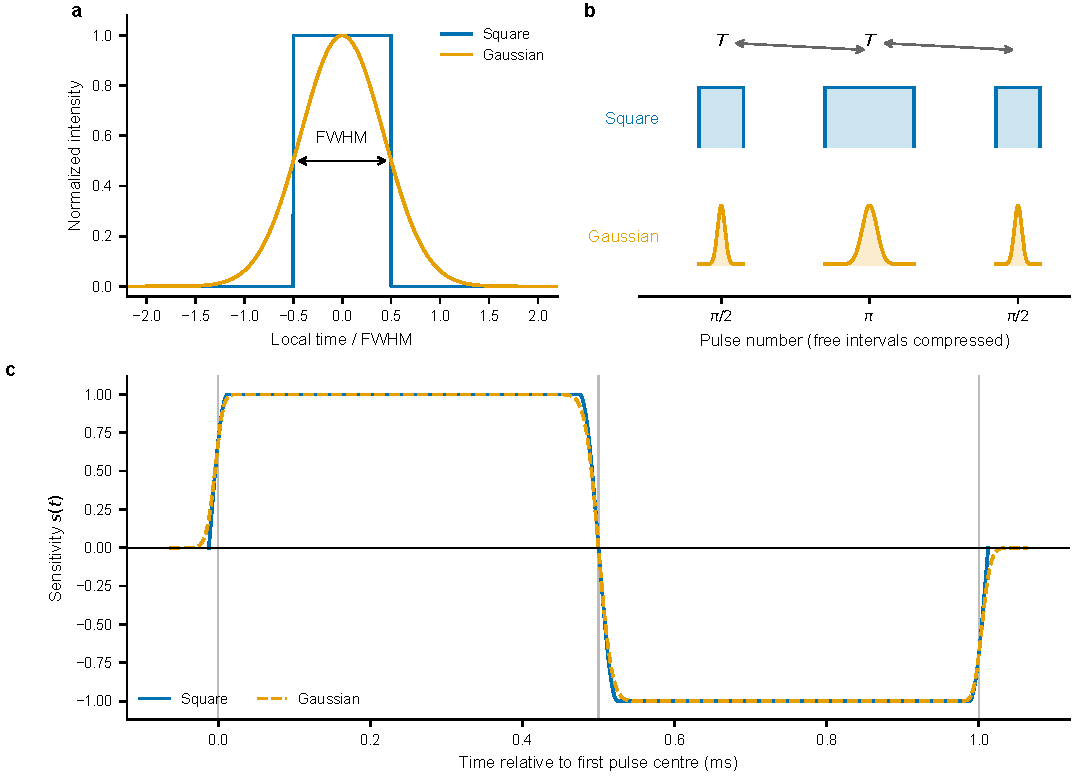
\includegraphics[width=\textwidth]{pulse_and_sensitivity.pdf}
\caption{Pulse envelopes and sensitivity functions. \textbf{a}, A square envelope and a Gaussian optical-intensity envelope with the same FWHM. \textbf{b}, Schematic $\pi/2$--$\pi$--$\pi/2$ sequences; free intervals are compressed. \textbf{c}, Sensitivity functions for illustrative centre separations of \SI{0.5}{\milli\second}, with $\tauhalf=\SI{25}{\micro\second}$ and $\taupi=\SI{50}{\micro\second}$. The square edge gap is converted so that the pulse centres coincide. The two shapes agree on the plateaus and differ only during the finite interactions.}
\label{fig:pulses}
\end{figure}

\section{Square-pulse calculation}

\subsection{Effective Rabi frequencies}

For a resonant square pulse, $\theta=\Omega\tau$. Independent $\pi/2$ and $\pi$ widths therefore imply
\begin{equation}
\boxed{\Omegahalf=\frac{\pi}{2\tauhalf},\qquad
\Omegapi=\frac{\pi}{\taupi}.}
\label{eq:squareRabi}
\end{equation}
The UI reports $\Omega/(2\pi)$ in hertz. If $\taupi=2\tauhalf$, both pulses have the same peak effective Rabi rate.

\subsection{Sensitivity function}

With the timing variables defined in \cref{sec:timing}, the square-pulse sensitivity function is
\begin{equation}
s_{\mathrm{sq}}(t)=
\begin{cases}
0, & t<0,\\
\sin(\Omegahalf t), & 0\leq t<\tauhalf,\\
1, & \tauhalf\leq t<t_2,\\
\cos[\Omegapi(t-t_2)], & t_2\leq t<t_2+\taupi,\\
-1, & t_2+\taupi\leq t<t_3,\\
-\cos[\Omegahalf(t-t_3)], & t_3\leq t<t_3+\tauhalf,\\
0, & t\geq t_3+\tauhalf.
\end{cases}
\label{eq:sSquare}
\end{equation}
Its derivative is non-zero only during the three pulses:
\begin{equation}
\dot{s}_{\mathrm{sq}}(t)=
\begin{cases}
\Omegahalf\cos(\Omegahalf t), & 0<t<\tauhalf,\\
-\Omegapi\sin[\Omegapi(t-t_2)], & t_2<t<t_2+\taupi,\\
\Omegahalf\sin[\Omegahalf(t-t_3)], & t_3<t<t_3+\tauhalf,\\
0, & \text{otherwise}.
\end{cases}
\label{eq:dsSquare}
\end{equation}
The integrals of these three pieces are $+1$, $-2$ and $+1$. Their sum is zero, which enforces $\Hphi(0)=0$.

\subsection{Stable analytic Fourier integral}

Direct formulas containing denominators $\omega\pm\Omega$ are formally singular at $\omega=\mp\Omega$, even though the physical limits are finite. The code avoids these removable singularities by defining
\begin{equation}
E(q,d)=d\,e^{iqd/2}\operatorname{sinc}\!\left(\frac{qd}{2}\right),
\qquad \operatorname{sinc}(x)=\frac{\sin x}{x}.
\end{equation}
The required local integrals are
\begin{align}
C(\omega,\Omega,d)&=\frac{E(\Omega-\omega,d)+E(-\Omega-\omega,d)}{2},\\
S(\omega,\Omega,d)&=\frac{E(\Omega-\omega,d)-E(-\Omega-\omega,d)}{2i}.
\end{align}
The complete square-pulse result is
\begin{equation}
\boxed{\begin{aligned}
\frac{\Hphi^{\mathrm{sq}}(\omega)}{n}
={}&\Omegahalf C(\omega,\Omegahalf,\tauhalf)
-\Omegapi e^{-i\omega t_2}S(\omega,\Omegapi,\taupi)\\
&+\Omegahalf e^{-i\omega t_3}S(\omega,\Omegahalf,\tauhalf)
\end{aligned}}
\label{eq:Hsquare}
\end{equation}
NumPy's \texttt{sinc} uses the normalized definition $\sin(\pi x)/(\pi x)$, so the code passes $qd/(2\pi)$ to obtain the mathematical definition used above.

\section{Gaussian-pulse calculation}

\subsection{Optical-intensity FWHM}

The Gaussian input width is defined as the full width at half maximum of the optical intensity:
\begin{equation}
I_j(t)=I_{0,j}\exp\left[-4\ln2\left(\frac{t-t_{c,j}}{\tau_j}\right)^2\right],
\label{eq:intensityGaussian}
\end{equation}
where $\tau_j$ is the entered FWHM. The corresponding standard deviation is
\begin{equation}
\sigma_j=\frac{\tau_j}{2\sqrt{2\ln2}}.
\end{equation}

The software assumes that the two counter-propagating Bragg fields have matched intensity envelopes. Their two-photon effective Rabi rate is then proportional to the product of their field amplitudes and therefore proportional to the common optical intensity envelope. Under this assumption,
\begin{equation}
\Omega_j(t)=\Omega_{0,j}\exp\left[-\frac{(t-t_{c,j})^2}{2\sigma_j^2}\right]
\end{equation}
has the same FWHM as \cref{eq:intensityGaussian}. For an ideal infinite Gaussian normalized to total area $\Theta_j$,
\begin{equation}
\boxed{\Omega_{0,j}=\frac{\Theta_j}{\sigma_j\sqrt{2\pi}}
=\frac{2\sqrt{\ln2}}{\sqrt{\pi}}\frac{\Theta_j}{\tau_j}.}
\label{eq:gaussianPeak}
\end{equation}

\begin{warningbox}[When optical-intensity FWHM is not the Rabi FWHM]
If only one Bragg beam is intensity-modulated while the other remains constant, the effective two-photon Rabi rate is proportional to the modulated field amplitude, $\sqrt{I(t)}$, rather than to $I(t)$. In that configuration the Rabi envelope has a different FWHM, and the current Gaussian conversion must be modified.
\end{warningbox}

\subsection{Finite numerical window and accumulated area}

The program truncates each Gaussian at $L_j=6\sigma_j$ and renormalizes it over $[-L_j,L_j]$. Writing $e_6=\operatorname{erf}(6/\sqrt{2})$, the implemented envelope and accumulated local area are
\begin{align}
\Omega_j(u)&=\frac{\Theta_j}{\sigma_j\sqrt{2\pi}\,e_6}
\exp\left(-\frac{u^2}{2\sigma_j^2}\right),\\
\theta_j(u)&=\Theta_j\frac{\operatorname{erf}[u/(\sqrt{2}\sigma_j)]+e_6}{2e_6},
\qquad -6\sigma_j\leq u\leq6\sigma_j.
\label{eq:gaussianArea}
\end{align}
This finite-window normalization makes $\theta_j(-6\sigma_j)=0$ and $\theta_j(6\sigma_j)=\Theta_j$ to numerical precision.

For separated pulses, the pulse-local sensitivity functions have the same rotation structure as the square case:
\begin{align}
s_1(t)&=\sin\theta_1(t), & \dot{s}_1(t)&=\Omega_1(t)\cos\theta_1(t),\\
s_2(t)&=\cos\theta_2(t), & \dot{s}_2(t)&=-\Omega_2(t)\sin\theta_2(t),\\
s_3(t)&=-\cos\theta_3(t), & \dot{s}_3(t)&=\Omega_3(t)\sin\theta_3(t).
\end{align}
The free-evolution plateaus remain $+1$ and $-1$. The Gaussian transfer function is then evaluated from \cref{eq:Hgeneral}.

\subsection{Gauss--Legendre quadrature}

Each pulse integral is mapped to the standard Gauss--Legendre interval. The code selects the number of nodes according to
\begin{equation}
N_q=\max\!\left[256,\left\lceil20f_{\max}\Delta t_j\right\rceil+64\right],
\end{equation}
where $\Delta t_j=12\sigma_j$ is the numerical pulse window. A hard limit of 4096 nodes prevents accidental calculations with unreasonable memory or runtime. Frequencies are processed in chunks of 2048, so a large frequency grid does not require one enormous complex-valued phase matrix.

The Gaussian calculation is numerical, but it is not a coarse time-grid FFT. It evaluates the requested frequencies directly and uses high-order quadrature inside each smooth pulse. This distinction avoids dependence on an arbitrary global time step and accurately represents very long free intervals through complex phase factors.

\section{Transfer functions and spectral densities}

\subsection{Magnitude, phase and power transfer}

If $S_{\Delta\varphi}(f)$ is the one-sided power spectral density (PSD) of the local differential optical phase, the atom-phase PSD is
\begin{equation}
\boxed{S_{\Phi_{\mathrm{AI}}}(f)=|\Hphi(f)|^2S_{\Delta\varphi}(f).}
\label{eq:PSD}
\end{equation}
For amplitude spectral density (ASD), the corresponding relation is
\begin{equation}
\sqrt{S_{\Phi_{\mathrm{AI}}}(f)}=|\Hphi(f)|\sqrt{S_{\Delta\varphi}(f)}.
\end{equation}
Thus ASD is multiplied by $|\Hphi|$, whereas PSD is multiplied by $|\Hphi|^2$. The present UI plots the former quantity. The complex transfer phase is calculated internally but is not displayed because its value depends on the chosen time origin; the magnitude is invariant under a global time translation.

\subsection{Sinusoidal frequency modulation}

For a deterministic laser-frequency modulation
\begin{equation}
\delta\nu(t)=\Delta\nu\cos(2\pi f_m t+\phi_0),
\end{equation}
the corresponding optical phase modulation follows from $\dot{\varphi}=2\pi\delta\nu$:
\begin{equation}
\delta\varphi(t)=\frac{\Delta\nu}{f_m}\sin(2\pi f_m t+\phi_0).
\end{equation}
The atom-phase peak amplitude is therefore
\begin{equation}
\Delta\Phi_{\mathrm{AI,pk}}=|\Hphi(f_m)|\frac{\Delta\nu}{f_m}.
\end{equation}
In a one-sided ideal PSD, the deterministic line has integrated power
\begin{equation}
\int_{\mathrm{line}}S_{\Phi_{\mathrm{AI}}}(f)\dd f
=\frac{1}{2}|\Hphi(f_m)|^2\left(\frac{\Delta\nu}{f_m}\right)^2.
\end{equation}
For a finite record, the line is broadened by the observation time and window function. Its integrated area, rather than its tallest PSD bin, is the stable quantity.

\begin{warningbox}[Common-mode frequency modulation]
The conversion above assumes that the modulation produces the differential phase $\Delta\varphi(t)$ seen by the atoms. A modulation applied to a common laser may cancel between the two Bragg fields or acquire an additional propagation-delay transfer function. Optical path difference, AOM architecture and which beam is modulated must be included before applying \cref{eq:PSD}.
\end{warningbox}

\section{Interpreting the plots}

\subsection{Sensitivity function}

The sensitivity function begins at zero, rises continuously to $+1$ during the first beam splitter, changes from $+1$ to $-1$ during the mirror pulse, and returns from $-1$ to zero during the final beam splitter. When $T$ is many orders of magnitude longer than the pulse widths, the full-sequence plot visually resembles an ideal step function. The pulse-shape differences remain present but are confined to very narrow regions. The first UI panel therefore uses compressed gaps to make the square or Gaussian envelopes and their FWHM values visible.

\subsection{Frequency fringes and the finite-pulse envelope}

In the instantaneous-pulse limit,
\begin{equation}
\Hphi(\omega)=n(1-e^{-i\omega T})^2,
\qquad |\Hphi|=4n\sin^2\left(\frac{\omega T}{2}\right).
\label{eq:instantaneous}
\end{equation}
The fringe period in ordinary frequency is approximately
\begin{equation}
\boxed{\Delta f_{\mathrm{fringe}}=\frac{1}{T}.}
\end{equation}
For $T=\SI{250}{\milli\second}$, the period is \SI{4}{\hertz}. This fine structure is produced by coherent addition of the three pulse contributions. A sinusoidal phase perturbation at a transfer-function zero is rejected, whereas one at a neighbouring maximum is transmitted strongly.

The pulse duration sets a separate, much higher frequency scale. When $f\ll1/\tau$, a perturbation changes little during a pulse and square and Gaussian responses are nearly identical. Their difference becomes clear near the effective Rabi frequency and above. Abrupt square edges produce slowly decaying Fourier side lobes, while the smooth Gaussian envelope suppresses high-frequency response more strongly.

\begin{figure}[H]
\centering
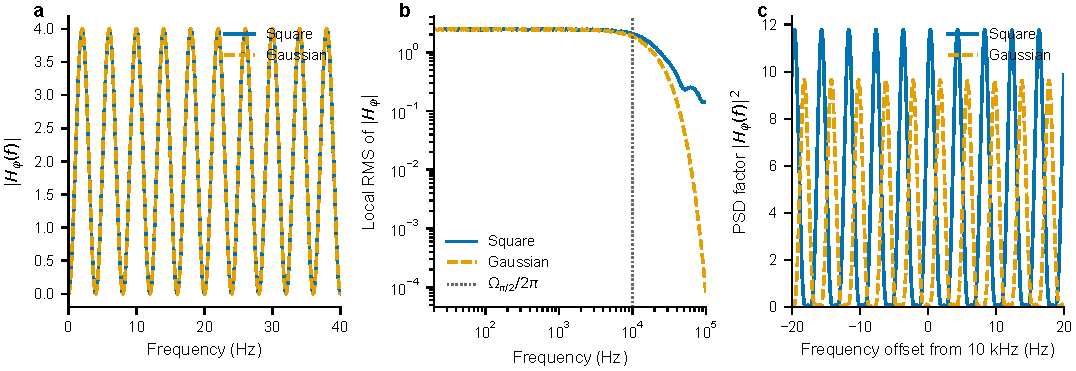
\includegraphics[width=\textwidth]{transfer_response.pdf}
\caption{Frequency response for $n=1$, $\tauhalf=\SI{25}{\micro\second}$, $\taupi=\SI{50}{\micro\second}$ and $T=\SI{250}{\milli\second}$. \textbf{a}, Resolved low-frequency magnitude; the \SI{4}{\hertz} fringe period is set by $1/T$. \textbf{b}, Local root-mean-square magnitude, obtained by averaging $|\Hphi|^2$ over one fringe period before taking the square root. The pulse shape controls the high-frequency envelope, and the dotted line marks $\Omegahalf/(2\pi)$ for the square pulse. \textbf{c}, Resolved PSD transfer factor in a \SI{40}{\hertz} interval around \SI{10}{\kilo\hertz}. At a specific coherent modulation frequency, the exact fringe value matters; for broadband noise, a local average is often more informative.}
\label{fig:transfer}
\end{figure}

\subsection{Sampling and apparent high-frequency disorder}

The UI uses a logarithmic frequency grid. At high frequency, adjacent logarithmic points may be separated by much more than $1/T$. Connecting those undersampled points can make a deterministic fringe pattern appear irregular or noisy. This is a plotting alias, not stochastic physics and not necessarily a quadrature error.

To resolve the fringes in a narrow interval, choose a linear-equivalent spacing satisfying approximately
\begin{equation}
\Delta f\lesssim\frac{1}{10T}.
\label{eq:resolution}
\end{equation}
The current UI always constructs a logarithmic grid, so the practical procedure is to narrow the frequency range around the region of interest and increase the number of points. For broadband PSD calculations over a very wide band, use a local average of $|\Hphi|^2$ or integrate the PSD directly rather than trying to draw every fringe.

\section{Detailed UI reference}

\subsection{Pulse-sequence controls}

\texttt{Pulse shape} selects the analytic square branch or numerical Gaussian branch. \texttt{Bragg order n} accepts positive integers only. The two pulse-width fields accept positive finite values in microseconds. The first and third $\pi/2$ pulses always share the same width. The \texttt{Interrogation time T} field remains in milliseconds in both modes, but its physical definition changes as described in \cref{sec:timing}.

The first panel displays normalized intensity, not absolute optical power. Relative peak heights follow the area normalization. For example, $\taupi=2\tauhalf$ gives equal square Rabi heights and, under the matched-envelope assumption, equal Gaussian peak Rabi rates. The FWHM arrows show the entered widths, and the blue arrows show $T$ using the correct edge or centre convention.

\subsection{Frequency controls}

The minimum frequency must be strictly positive because the plot uses a logarithmic axis. The DC value is nevertheless evaluated in the self-tests and enforced exactly as $\Hphi(0)=0$. The maximum frequency must exceed the minimum. A very high maximum frequency combined with a broad Gaussian pulse may exceed the 4096-node quadrature safeguard; the UI then asks for a lower maximum frequency or a narrower pulse.

The point count controls only the requested frequency grid. It does not change the internal Gauss--Legendre order used inside Gaussian pulses. More points therefore improve displayed frequency resolution without changing the pulse-integration method.

\subsection{Displayed status information}

The status block reports the plotted sequence duration, peak effective Rabi rates, the active definition of $T$, the analytic or numerical integration branch, and the DC identity. In Gaussian mode the sequence duration includes the $\pm6\sigma$ numerical windows. It is a plotting and integration extent, not a statement that a physical Gaussian field becomes exactly zero at those times.

\subsection{Saving and inspecting figures}

The Matplotlib toolbar provides zoom, pan, coordinate inspection and view reset. In the compressed pulse panel, the cursor readout converts the schematic coordinate back to relative physical time. The first pulse centre is the time origin. PDF or SVG export is preferred for reports because the line art remains vector-based; PNG is useful for slides or quick sharing.

\section{Worked examples}

\subsection{Default first-order calculation}

Set $n=1$, $\tauhalf=\SI{25}{\micro\second}$, $\taupi=\SI{50}{\micro\second}$ and $T=\SI{250}{\milli\second}$. In square mode, \cref{eq:squareRabi} gives
\begin{equation}
\frac{\Omegahalf}{2\pi}=\frac{1}{4\tauhalf}=\SI{10}{\kilo\hertz},
\qquad
\frac{\Omegapi}{2\pi}=\frac{1}{2\taupi}=\SI{10}{\kilo\hertz}.
\end{equation}
The transfer fringes repeat every \SI{4}{\hertz}. Finite-pulse filtering becomes prominent near the \SI{10}{\kilo\hertz} Rabi scale.

In Gaussian mode, the same entered FWHM values and matched-intensity assumption give, from \cref{eq:gaussianPeak},
\begin{equation}
\frac{\Omega_{0,\pi/2}}{2\pi}
=\frac{\Omega_{0,\pi}}{2\pi}
\simeq\SI{9.394}{\kilo\hertz}.
\end{equation}
The low-frequency response remains nearly identical because the pulse areas and centre separation dominate there. The Gaussian high-frequency envelope decreases more rapidly.

\subsection{Changing Bragg order}

Changing $n$ from 1 to 3 leaves $s(t)$ unchanged. The plotted magnitude triples and the PSD transfer factor increases by nine:
\begin{equation}
|\Hphi^{(3)}|=3|\Hphi^{(1)}|,
\qquad
|\Hphi^{(3)}|^2=9|\Hphi^{(1)}|^2.
\end{equation}
This scaling is a phase-gain convention, not a full prediction of third-order Bragg diffraction efficiency.

\subsection{Evaluating a modulation line}

Suppose a differential frequency modulation has peak deviation $\Delta\nu=\SI{10}{\hertz}$ at $f_m=\SI{100}{\hertz}$. Its phase-modulation peak is $\Delta\nu/f_m=\SI{0.1}{\radian}$. If the UI gives $|\Hphi(f_m)|=2.5$, the atom-phase peak is \SI{0.25}{\radian}, and the integrated one-sided PSD line power is $0.25^2/2=\SI{0.03125}{\radian\squared}$.

\section{Validation and reproducibility}

Run the built-in test suite without opening the GUI:
\begin{lstlisting}[language=bash]
python "bragg_transfer_function_ui.py" --self-test
\end{lstlisting}

\begin{table}[H]
\centering
\caption{Automated checks implemented by the application.}
\begin{tabularx}{\textwidth}{@{}lX@{}}
\toprule
Check & Purpose \\
\midrule
Exact DC response & Enforces $\Hphi(0)=0$ for a closed interferometer sequence. \\
Sensitivity boundaries & Confirms $0\rightarrow+1\rightarrow-1\rightarrow0$ at all pulse boundaries. \\
Square analytic/numerical comparison & Compares the stable analytic expression with a high-resolution trapezoidal reference. \\
Rabi-frequency regularity & Confirms finite values at removable singularities $\omega=\pm\Omega$. \\
Pulse-area changes & Confirms Gaussian derivative integrals $+1,-2,+1$. \\
Bragg-order scaling & Confirms linear scaling of complex $\Hphi$ with $n$. \\
Instantaneous limit & Confirms convergence toward $4n\sin^2(\omega T/2)$ as pulse widths vanish. \\
GUI smoke tests & Confirms that both pulse modes construct and plot without callback errors. \\
\bottomrule
\end{tabularx}
\end{table}

The manual figures can be regenerated with
\begin{lstlisting}[language=bash]
python "manual_figures.py"
\end{lstlisting}
This command writes vector PDF files into \texttt{figures/}. It uses the same calculation functions as the GUI, ensuring that equations, examples and plotted results remain synchronized with the application.

\begin{checkbox}[Required physical identities]
For every valid parameter set, verify $s(-\infty)=s(+\infty)=0$, $\Hphi(0)=0$, linear $n$ scaling and convergence to the instantaneous-pulse result when the widths become negligible compared with $T$.
\end{checkbox}

\section{Troubleshooting}

\begin{longtable}{@{}p{0.29\textwidth}p{0.65\textwidth}@{}}
\toprule
Symptom & Explanation and remedy \\
\midrule
\endhead
The high-frequency curve looks random. & The logarithmic grid undersamples fringes spaced by approximately $1/T$. Narrow the frequency interval and increase the point count, or use a locally averaged PSD factor. \\
Square and Gaussian curves look almost identical. & This is expected below the inverse pulse duration. Compare their high-frequency envelopes or use wider pulses while keeping the pulse areas normalized. \\
Gaussian calculation reports overlapping pulses. & The $\pm6\sigma$ numerical windows overlap. Increase centre spacing $T$ or use a full overlapping-pulse Hamiltonian, which is outside this application. \\
Gaussian calculation requests too many quadrature nodes. & Reduce $f_{\max}$ or use a narrower pulse. The 4096-node limit prevents excessive runtime and memory use. \\
The sensitivity transitions are invisible. & The full sequence time is much longer than the pulse widths. Use the compressed pulse panel to inspect FWHM and shape; zoom around a pulse in the sensitivity panel if needed. \\
Changing $n$ does not alter $s(t)$. & This is intentional. The MIGA factor $n$ multiplies the phase transfer function outside the normalized sensitivity function. \\
The inferred frequency-noise response is too large or too small. & Confirm that the input is the differential phase at the atoms. Common-mode rejection, optical delay and AOM topology are not included automatically. \\
\bottomrule
\end{longtable}

\section{Known limitations and extension path}

The current software is deliberately a reduced model. It is reliable for ideal resonant, separated pulses that can be described by a two-level rotation with a known effective Rabi envelope. The following effects require a more complete treatment:

\begin{itemize}
  \item detuning and Doppler-dependent velocity distributions;
  \item simultaneous coupling of multiple momentum states in higher-order Bragg diffraction;
  \item non-ideal diffraction efficiency and parasitic interferometers;
  \item AC Stark shifts, spontaneous emission and laser-intensity noise;
  \item optical-cavity build-up, cavity pole filtering and propagation delay;
  \item overlapping pulses or arbitrary chirped/phase-shaped envelopes;
  \item correlations between the two optical fields and spatial phase variations across the atomic cloud.
\end{itemize}

The natural extension is to propagate the full time-dependent Hamiltonian, compute the interferometer output phase under a small phase perturbation, and obtain the sensitivity function by functional differentiation. The present UI, plotting and PSD layers can then be retained while replacing the pulse-dynamics backend.

\section{Code organization}

The application is intentionally distributed as a single executable Python file. \path{InterferometerParameters} validates SI-valued parameters and defines the square schedule. \path{sensitivity_function} and \path{transfer_function} implement the square branch. \path{gaussian_sensitivity_function} and \path{gaussian_transfer_function} implement the Gaussian branch. \path{BraggTransferFunctionApp} owns the Tkinter controls and Matplotlib canvas. The \path{run_self_test} function provides a dependency-free validation entry point.

All physical calculations use seconds, hertz and radians internally. Unit conversion occurs only when values are read from the UI or reported to the user. This separation prevents microsecond/millisecond conversion errors from propagating into the model.

\section{Using this manual on Overleaf}

Upload \texttt{bragg\_transfer\_function\_manual.tex} together with the \texttt{figures/} directory. Set the main document to the manual file and compile with pdfLaTeX. The document uses packages included in current TeX Live and Overleaf distributions, including \texttt{newtx}, \texttt{fontawesome5}, \texttt{tcolorbox}, \texttt{tikz}, \texttt{siunitx} and \texttt{cleveref}. No shell escape, external bibliography processor or custom font upload is required.

The source is a technical manual with Nature-inspired typography, accessible prose, numbered references, double-column-width vector figures and colorblind-safe colors. It is not an official Nature template and should not be submitted as a journal manuscript without adapting it to the current instructions of the target Nature Portfolio journal.

\section*{Code availability}

The calculator, manual source and figure-generation script are maintained in the MIGA programme repository at
\begin{center}
\href{https://github.com/Quantum00man/MIGA-program/tree/main/bragg\%20transfer\%20function}{github.com/Quantum00man/MIGA-program/tree/main/bragg-transfer-function}.
\end{center}

\begin{thebibliography}{9}

\bibitem{Canuel2018}
Canuel, B. \textit{et al.} Exploring gravity with the MIGA large scale atom interferometer. \textit{Sci. Rep.} \textbf{8}, 14064 (2018). \href{https://doi.org/10.1038/s41598-018-32165-z}{doi:10.1038/s41598-018-32165-z}.

\bibitem{Cheinet2008}
Cheinet, P., Canuel, B., Pereira Dos Santos, F., Gauguet, A., Yver-Leduc, F. \& Landragin, A. Measurement of the sensitivity function in a time-domain atomic interferometer. \textit{IEEE Trans. Instrum. Meas.} \textbf{57}, 1141--1148 (2008). \href{https://doi.org/10.1109/TIM.2007.915148}{doi:10.1109/TIM.2007.915148}.

\end{thebibliography}

\end{document}
